\documentclass[11pt,a4paper,oneside,openany,indonesian]{report}
\usepackage[a4paper,top=25mm,bottom=25mm,left=30mm,right=25mm,headheight=16pt,headsep=7mm,footskip=12mm]{geometry}
\usepackage{iftex}
\ifLuaTeX
  \usepackage[bidi=basic,shorthands=off,provide=*]{babel}
\else
  \usepackage[bidi=default,shorthands=off,provide=*]{babel}
\fi
\ifPDFTeX\else\babelfont{rm}[]{Charter}\fi
\usepackage{hyperref}
% Shared preamble for the Jakarta TGA chapters.
\usepackage{xcolor}
\usepackage{graphicx}
\usepackage{amsmath,amssymb}
\usepackage{iftex}
\ifPDFTeX
  \usepackage[T1]{fontenc}
  \usepackage[utf8]{inputenc}
  \usepackage{textcomp}
\else
  \usepackage{unicode-math}
  \defaultfontfeatures{Scale=MatchLowercase}
  \defaultfontfeatures[\rmfamily]{Ligatures=TeX,Scale=1}
\fi
\usepackage{lmodern}
\ifPDFTeX\else
  \setmainfont[]{Times New Roman}
  \setsansfont[]{Arial}
  \IfFontExistsTF{Consolas}{\setmonofont[]{Consolas}}{\setmonofont[]{Courier New}}
\fi
\IfFileExists{microtype.sty}{\usepackage{microtype}}{}
\usepackage{longtable,booktabs,array,tabularx,adjustbox,calc}
\usepackage{pdflscape}
\usepackage{caption}
\captionsetup[table]{skip=6pt}
\newcounter{none}
\usepackage{float}
\usepackage{setspace}
\usepackage{ragged2e}
\usepackage{titlesec}
\usepackage{enumitem}
\usepackage{needspace}
\usepackage{fancyhdr}
\usepackage{newunicodechar}
\usepackage{bookmark}
\usepackage{xurl}
\usepackage{csquotes}
\usepackage[backend=biber,style=authoryear,maxcitenames=2,maxbibnames=99,uniquelist=false,uniquename=false]{biblatex}
\DeclareLanguageMapping{indonesian}{english}
\DefineBibliographyStrings{english}{and={dan},andothers={dkk\adddot}}
\DefineBibliographyStrings{indonesian}{and={dan},andothers={dkk\adddot}}
\AtBeginDocument{\renewcommand*{\finalnamedelim}{\addspace dan\space}}
\addbibresource{references.bib}
\DeclareFieldFormat{title}{#1}
\DeclareFieldFormat[article,inbook,incollection,inproceedings,inreference,patent,thesis,unpublished]{title}{#1}
\AtBeginBibliography{\small\setlength{\bibitemsep}{0.15em}}

\newunicodechar{∅}{\ensuremath{\varnothing}}

% Placeholder untuk gambar yang dibuat manual (peta GIS). Ganti dengan \includegraphics setelah berkas target tersedia.
\newcommand{\GambarPlaceholder}[2][7cm]{%
  \fbox{\parbox[c][#1][c]{0.92\linewidth}{\centering\small
    \textbf{PLACEHOLDER GAMBAR}\\[0.6em]#2}}}

\definecolor{Ink}{HTML}{222222}
\definecolor{RuleGray}{HTML}{666666}

\AtBeginDocument{%
  \hypersetup{linkcolor=Ink,citecolor=Ink,urlcolor=Ink,pdfborder={0 0 0}}%
  \urlstyle{same}%
}

\setstretch{1.5}
\setlength{\parindent}{1.1em}
\setlength{\parskip}{0.28em}
\setlength{\emergencystretch}{2.5em}
\clubpenalty=10000
\widowpenalty=10000
\displaywidowpenalty=10000
\raggedbottom

\setlist[itemize]{leftmargin=1.7em,itemsep=0.25em,topsep=0.35em}
\setlist[enumerate]{leftmargin=1.9em,itemsep=0.25em,topsep=0.35em}

\titleformat{\chapter}[display]
  {\normalfont\bfseries\centering\color{Ink}}
  {}{0pt}{\Large\hyphenpenalty=10000\exhyphenpenalty=10000}
\titlespacing*{\chapter}{0pt}{-6pt}{18pt}
\titleformat{\section}{\Needspace{4\baselineskip}\large\bfseries\color{Ink}}{\thesection}{0.7em}{}
\titleformat{\subsection}{\Needspace{3\baselineskip}\normalsize\bfseries\color{Ink}}{\thesubsection}{0.7em}{}
\titleformat{\subsubsection}{\Needspace{3\baselineskip}\normalsize\bfseries\color{Ink}}{\thesubsubsection}{0.7em}{}

\pagestyle{plain}
\fancyhf{}
\fancyfoot[C]{\thepage}
\renewcommand{\headrulewidth}{0pt}
\renewcommand{\footrulewidth}{0pt}
\fancypagestyle{plain}{%
  \fancyhf{}
  \fancyfoot[C]{\thepage}
  \renewcommand{\headrulewidth}{0pt}
}

\renewcommand{\arraystretch}{1.2}
\setlength{\extrarowheight}{1pt}
\setlength{\tabcolsep}{4pt}
\providecommand{\tightlist}{\setlength{\itemsep}{0pt}\setlength{\parskip}{0pt}}
\setlength{\LTpre}{0.5em}
\setlength{\LTpost}{0.8em}
\AtBeginEnvironment{longtable}{\footnotesize\setstretch{1.0}\setlength{\tabcolsep}{3pt}\setlength{\extrarowheight}{1pt}}
\AtBeginEnvironment{table}{\setstretch{1.0}}
\AtBeginEnvironment{figure}{\setstretch{1.0}}
\AtBeginEnvironment{quote}{\small\setlength{\leftskip}{1.2em}\setlength{\rightskip}{1.2em}}


\hypersetup{
  pdftitle={Bab 1 Pendahuluan},
  pdfauthor={Mahastri Laksita Sam Widita},
  pdflang={id-ID},
  hidelinks
}

\title{\textbf{Borrowed Size atau Agglomeration Shadow?}\\[0.4em]
Analisis Hubungan Integrasi Metropolitan dengan Kematangan Pusat-Pusat Sekunder di Kawasan Aglomerasi Jakarta}
\providecommand{\subtitle}[1]{\gdef\thesubtitle{#1}}
\subtitle{Bab 1 Pendahuluan}
\author{Mahastri Laksita Sam Widita\\NIM 22/503065/TK/54947\\[0.5em]
Pembimbing: Rendy Bayu Aditya\\[0.5em]
Program Studi Perencanaan Wilayah dan Kota\\
Departemen Teknik Arsitektur dan Perencanaan\\
Fakultas Teknik\\
Universitas Gadjah Mada}
\date{Kabupaten Sleman, Daerah Istimewa Yogyakarta\\2026}

\makeatletter
\renewcommand{\maketitle}{%
  \begin{titlepage}
    \centering
    {\Large\bfseries TUGAS AKHIR\par}
    \vfill
    {\LARGE\bfseries \@title\par}
    \vspace{1.2cm}
    {\large \thesubtitle\par}
    \vfill
    {\large \@author\par}
    \vfill
    {\large \@date\par}
  \end{titlepage}}
\makeatother

\begin{document}
\maketitle
\tableofcontents
\clearpage

\chapter{Pendahuluan}

\section{Latar belakang}

Perkembangan metropolitan Jakarta tidak berhenti pada batas administratif DKI Jakarta. Permukiman, kawasan industri, pusat pelayanan, dan jaringan transportasi berkembang di wilayah sekitarnya, sementara perjalanan penduduk dan kegiatan ekonomi menghubungkan berbagai bagian kawasan tersebut. Jakarta tetap menjadi pusat dominan, tetapi sejumlah kawasan di sekitarnya telah menjadi konsentrasi penduduk, pekerjaan, industri, dan pelayanan. Kajian mengenai Jabotabek dan Jabodetabek mencatat pergeseran kegiatan ke pinggiran, perkembangan kota baru dan kawasan industri, serta arus komuter antarpinggiran \parencite{henderson1996,hudalahfirman2012,hudalahetal2013,sadewoetal2023}.

Keberadaan beberapa konsentrasi di luar Jakarta belum menunjukkan sistem metropolitan yang seimbang. Polisentrisitas morfologis, yang terlihat dari persebaran konsentrasi penduduk atau pekerjaan, berbeda dari polisentrisitas fungsional yang terbentuk melalui arus dan interaksi antarpusat \parencite{burgermeijers2012}. Suatu kawasan dapat mempunyai banyak pusat secara fisik, tetapi hubungan fungsionalnya tetap terpusat, hierarkis, atau terfragmentasi. Hubungan yang kuat dengan Jakarta juga tidak selalu berarti ketergantungan sepihak. Pusat sekunder dapat menarik pekerja, melayani pasar yang lebih luas, atau berhubungan langsung dengan pusat sekunder lain. Analisis karena itu harus mempertahankan arah dan asimetri relasi, alih-alih mereduksinya sejak awal menjadi satu skor keterhubungan.

Persoalan berikutnya adalah apakah pertumbuhan pusat-pusat di sekitar Jakarta diikuti oleh penguatan fungsi lokal. Pertambahan penduduk, luas kawasan terbangun, fasilitas, atau pekerjaan menunjukkan dimensi perkembangan yang berbeda. Dekonsentrasi manufaktur, misalnya, dapat meningkatkan jumlah pekerjaan di pinggiran tanpa diikuti perpindahan fungsi keputusan, layanan bisnis, atau layanan berorde tinggi. Literatur mengenai spesialisasi fungsional menunjukkan bahwa produksi dapat tersebar ke kota yang lebih kecil ketika fungsi pengendalian dan layanan strategis tetap terkonsentrasi di kota besar \parencite{durantonpuga2005}. Dalam konteks Jabodetabek, pertumbuhan kawasan industri atau kota baru karena itu tidak cukup untuk menyimpulkan bahwa suatu pusat telah matang pada seluruh domain fungsi.

Perbedaan antara ukuran lokal dan fungsi aktual menjadi dasar konsep \emph{borrowed size}. Konsep ini menjelaskan kemungkinan bahwa kota atau pusat yang lebih kecil memperoleh fungsi atau kinerja yang biasanya diasosiasikan dengan kota lebih besar melalui relasinya dengan pusat lain. Namun, kedekatan geografis tidak cukup untuk membuktikan peminjaman ukuran. Relasi perlu ditunjukkan melalui arus atau interaksi, sedangkan fungsi aktual perlu dibandingkan dengan fungsi yang secara wajar diharapkan berdasarkan massa dan karakteristik lokal \parencite{meijersburger2017,meijersetal2016}. Surplus fungsi relatif yang tidak disertai bukti relasional belum dapat disebut \emph{borrowed size}.

Hubungan dengan pusat dominan juga dapat berkaitan dengan hasil yang kurang menguntungkan. Kompetisi atas tenaga kerja, permintaan, investasi, dan fungsi berorde tinggi dapat membuat pusat sekunder tetap berada di bawah tingkat fungsi yang diharapkan. Pola tersebut sering dibahas melalui konsep \emph{agglomeration shadow}. Meskipun demikian, bukti empiris tidak menunjukkan satu tanda hubungan yang berlaku umum. Manfaat jaringan, defisit fungsi, dan hasil campuran berubah menurut ukuran pusat, sektor, posisi jaringan, hierarki, dan skala analisis \parencite{volgmannrusche2020,yangzhudu2022,zhenshilu2023}. Temuan tandingan juga menunjukkan bahwa kedekatan dengan kota besar dapat berkaitan dengan pertumbuhan wilayah sekitarnya, sehingga \emph{shadow} tidak boleh diasumsikan sebelum analisis dilakukan \parencite{partridgeetal2009,sunding2016}.

Perbedaan hasil antardomain sangat mungkin muncul di Jabodetabek. Sebuah pusat dapat mempunyai surplus pekerjaan manufaktur sekaligus defisit layanan tingkat tinggi. Penduduknya mungkin memperoleh akses ke pasar kerja metropolitan sambil menanggung waktu dan biaya perjalanan yang besar. Pekerjaan yang berada di suatu pusat pun belum tentu dinikmati oleh penduduk setempat. Kajian komuter dan akses pekerjaan di Jakarta menunjukkan bahwa manfaat akses, penggunaan aktual, persaingan antarpencari kerja, dan beban perjalanan adalah objek yang berbeda \parencite{andani2021,aritenang2022,andani2025}. Manfaat, beban, dan ketergantungan karena itu tidak dilebur menjadi satu skor bersih. Analisis harus tetap menunjukkan penerima manfaat dan penanggung beban.

Literatur internasional membahas fungsi pinjaman, kinerja pinjaman, dan \emph{agglomeration shadow}. Penelitian Jabodetabek telah menguraikan dekonsentrasi industri, perkembangan kota baru, perubahan struktur metropolitan, komuter, akses pekerjaan, dan fragmentasi tata kelola. Dalam korpus yang ditelusuri, pembahasan tersebut belum dirangkai dalam satu pengukuran yang mempertahankan arah relasi metropolitan, membandingkan fungsi aktual per domain dengan ekspektasi dari massa lokal, memisahkan manfaat dari beban menurut aktor dan lokasi, serta menguji ketahanan hasil terhadap keputusan analitis. Pernyataan ini hanya berlaku pada korpus yang diperiksa; ia tidak menyatakan bahwa susunan penelitian serupa belum pernah dibuat.

Penelitian ini tidak memilih \emph{borrowed size} atau \emph{agglomeration shadow} sebagai jawaban awal. Kedua konsep dipakai untuk menafsirkan konfigurasi observasional setelah relasi metropolitan, fungsi relatif, dan penjelasan alternatif diperiksa. Objek yang diestimasi adalah hubungan antara relasi metropolitan terarah suatu pusat sekunder dan deviasi fungsi aktual dari fungsi yang diharapkan menurut massa serta karakteristik lokal. Pengukuran dilakukan per domain agar surplus pada satu domain tidak menutupi defisit pada domain lain.

Penelitian ini berfokus pada pusat-pusat sekunder di Kawasan Aglomerasi Jakarta. DKI Jakarta diperlakukan sebagai satu inti pada spesifikasi utama untuk membaca hubungan eksternal dan tanggung jawab administratif, tetapi kemungkinan bahwa arus menuju subpusat yang berbeda di dalam DKI akan diperiksa sebagai spesifikasi alternatif. Batas administratif tetap dipertahankan sebagai batas kewenangan, pelayanan, dan tanggung jawab pemerintah. Jejak fungsional yang melintasi batas dibaca sebagai hubungan metropolitan, bukan sebagai perluasan yurisdiksi Jakarta.

Penelitian ini tidak mengajukan konsep baru dan tidak menganggap integrasi selalu menguntungkan atau merugikan. Sumbangan penelitian terletak pada penyatuan lima operasi: mengukur relasi terarah, membentuk tolok ukur fungsi dari massa lokal, menganalisis hubungan per domain, memisahkan manfaat dari beban, dan memeriksa ketahanan hasil. Tipologi hanya menjadi ringkasan akhir jika profil kontinu dan ketidakpastiannya telah diperiksa.

Pemilihan data merupakan bagian dari rancangan pengukuran. Penelitian ini menggunakan proksi dan sumber terbuka untuk membentuk informasi lokasi, fungsi, dan hubungan metropolitan. Sumber administratif terbuka, peta kolaboratif, direktori usaha dan fasilitas, informasi transportasi, serta penginderaan jauh dinilai dari kesesuaiannya dengan pertanyaan penelitian. Sumber alternatif dapat lebih tepat daripada data agregat yang tersedia, tetapi keunggulan itu harus dibuktikan untuk setiap konstruk, wilayah, dan periode.

\begin{figure}[H]
  \centering
  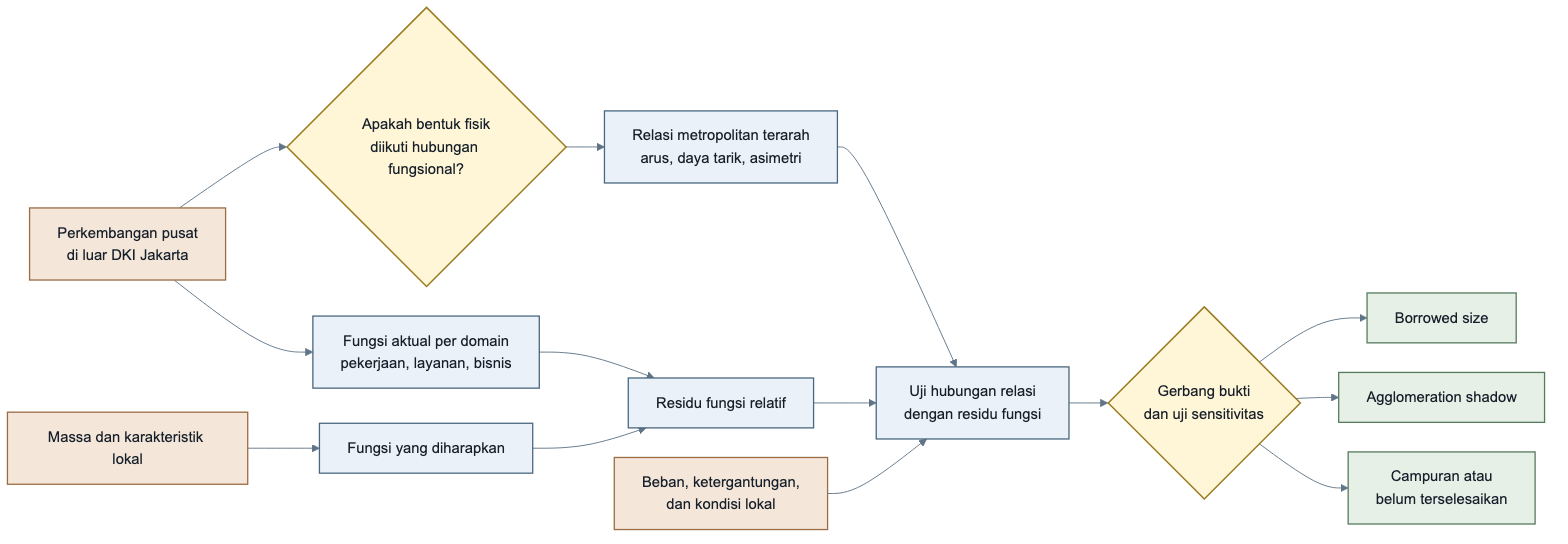
\includegraphics[width=\textwidth]{figures/bab1_logika_penelitian.png}
  \caption{Logika masalah dan objek pengukuran penelitian. Diagram merangkum hubungan antara perkembangan pusat di luar DKI Jakarta, relasi metropolitan terarah, fungsi relatif, beban, dan gerbang interpretasi.}
  \label{fig:bab1-logika}
\end{figure}

\section{Rumusan masalah}

Transformasi metropolitan Jakarta telah membentuk pusat kegiatan di luar inti administratif. Keberadaan pusat tersebut belum menjelaskan kualitas relasinya dengan Jakarta ataupun kekuatan fungsi lokalnya. Hubungan metropolitan dapat berkaitan dengan surplus fungsi pada satu domain, defisit pada domain lain, manfaat akses, beban perjalanan, atau ketergantungan yang asimetris. Masalah penelitian terletak pada konfigurasi hubungan dan fungsi relatif yang teramati pada setiap pusat.

Pertanyaan utama penelitian adalah:

\begin{quote}
Bagaimana hubungan metropolitan terarah berkaitan dengan fungsi relatif pusat-pusat sekunder di Kawasan Aglomerasi Jakarta, dan dalam kondisi apa hubungan tersebut menunjukkan konfigurasi surplus fungsi, defisit fungsi, manfaat akses, beban, ketergantungan, atau hasil campuran?
\end{quote}

Pertanyaan utama tersebut dijabarkan menjadi empat pertanyaan penelitian:

\begin{enumerate}
  \item Bagaimana arah, intensitas, dan asimetri relasi pusat-pusat sekunder dengan Jakarta serta dengan pusat sekunder lain berdasarkan pengamatan dan estimasi dari sumber terbuka?
  \item Pada setiap domain fungsi yang diteliti, bagaimana fungsi suatu pusat yang diukur atau diestimasi dibandingkan dengan fungsi yang diharapkan berdasarkan massa dan karakteristik lokal, serta bagaimana perbandingan tersebut berubah pada indikator yang memiliki seri sebanding?
  \item Bagaimana dimensi relasi metropolitan terarah berasosiasi dengan surplus atau defisit fungsi relatif pada setiap domain, setelah tumpang tindih antarkonstruk dan penjelasan alternatif yang relevan diperiksa?
  \item Bagaimana spesialisasi fungsi, hierarki, status administratif, posisi jaringan, dan kondisi lokal membedakan hubungan, manfaat, beban, ketergantungan, serta konfigurasi hasil antarpusat?
\end{enumerate}

Analisis sensitivitas tidak ditempatkan sebagai pertanyaan substantif yang berdiri sendiri. Analisis tersebut digunakan untuk menilai kepercayaan terhadap jawaban keempat pertanyaan melalui perubahan unit, delineasi, indikator, transformasi, tolok ukur, bobot, ambang, dan spesifikasi yang masih mengestimasi objek sejenis. Perubahan sumber atau konstruk yang menghasilkan estimand berbeda dilaporkan sebagai triangulasi atau perubahan estimand, bukan sebagai sensitivitas model yang ekuivalen.

\section{Tujuan penelitian}

Tujuan umum penelitian ini adalah menganalisis hubungan antara relasi metropolitan terarah dan fungsi relatif pusat-pusat sekunder di Kawasan Aglomerasi Jakarta secara multidimensi, dengan membedakan domain fungsi, penerima manfaat, penanggung beban, serta ketahanan hasil terhadap keputusan analitis.

Tujuan khusus penelitian adalah:

\begin{enumerate}
  \item mengukur dan memetakan arah, intensitas, serta asimetri relasi pusat-pusat sekunder dengan Jakarta dan dengan pusat sekunder lain;
  \item mengukur atau mengestimasi fungsi per domain, membandingkannya dengan ekspektasi berdasarkan massa serta karakteristik lokal, dan membaca perubahannya pada indikator dengan seri sebanding;
  \item menguji asosiasi antara dimensi relasi metropolitan terarah dan surplus atau defisit fungsi relatif per domain dengan memperhatikan ketidakpastian serta penjelasan alternatif;
  \item menjelaskan perbedaan konfigurasi hubungan, manfaat, beban, ketergantungan, dan fungsi relatif menurut spesialisasi fungsi, hierarki, status administratif, posisi jaringan, serta kondisi lokal; dan
  \item menilai ketahanan temuan melalui analisis sensitivitas yang sesuai serta menyajikan tipologi ringkas hanya apabila pola, ambang, dan stabilitas empirisnya memadai.
\end{enumerate}

\section{Batasan penelitian}

Penelitian ini dibatasi pada sistem Jabodetabek administratif yang mencakup DKI Jakarta, Kabupaten Bogor, Kota Bogor, Kota Depok, Kabupaten Tangerang, Kota Tangerang, Kota Tangerang Selatan, Kabupaten Bekasi, dan Kota Bekasi. Batas tersebut digunakan sebagai ruang kerja utama dan tidak menyatakan bahwa batas administratif identik dengan batas fungsional metropolitan. Wilayah di luar cakupan dapat digunakan sebagai pembanding hanya apabila definisi, unit, dan periodenya kompatibel.

Unit substantif penelitian adalah kandidat pusat sekunder beserta wilayah tangkapan fungsionalnya. Unit perhitungan dapat berupa kecamatan, beberapa unit yang bersebelahan, zona asal-tujuan, titik fasilitas, atau sel raster sesuai resolusi sumber yang dapat dipertanggungjawabkan. Nilai kabupaten/kota tidak diturunkan ke kecamatan atau titik tanpa model eksplisit, asumsi yang terlihat, pemeriksaan independen, dan pelabelan sebagai estimasi.

Penelitian bertumpu pada proksi dan sumber terbuka. Data pemerintah terbuka dapat digunakan apabila sesuai, sedangkan data tertutup, permohonan kelembagaan, sensus usaha lengkap, data ponsel individu, atau matriks OD mikro bukan syarat rancangan. Ketersediaan koordinat, panjang seri, dan banyaknya sumber tidak otomatis membuktikan mutu pengukuran. Setiap proksi dinilai berdasarkan kesesuaian konstruk, cakupan spasial dan temporal, keterulangan, biaya pemerolehan, lisensi, dan hasil pemeriksaan independen.

Desain waktu bersifat multitemporal sesuai bukti. Perubahan hanya dianalisis pada indikator yang memiliki seri sebanding; indikator lain digunakan pada periode yang tersedia dengan tahun observasi yang ditulis jelas. Perubahan keterlihatan digital, perubahan kategori, dan perubahan batas tidak boleh diperlakukan otomatis sebagai perubahan fenomena. Panel lengkap dengan satu tahun jangkar untuk seluruh sumber tidak diasumsikan.

Fungsi yang dianalisis dibatasi pada domain yang memiliki pengukuran atau proksi yang dapat dipertanggungjawabkan, seperti pekerjaan dan struktur sektor, layanan lokal, layanan berorde tinggi, serta fungsi bisnis atau keputusan. Jumlah titik usaha tidak disebut produktivitas, pendapatan, inovasi, atau kesejahteraan tanpa pengukuran atau model yang sesuai. Estimasi pekerjaan, aksesibilitas, dan relasi asal-tujuan dilaporkan bersama asumsi, rentang, serta ketidakpastiannya. CCTV dan SUMO hanya digunakan jika audit kelayakan, privasi, cakupan, dan kalibrasi memadai.

Hasil penelitian bersifat observasional dan asosiasional. Penelitian ini tidak mengidentifikasi pengaruh kausal Jakarta terhadap pusat sekunder, tidak menetapkan satu radius metropolitan yang benar, tidak menjamin bahwa setiap pusat akan masuk tipologi tertentu, dan tidak memprediksi dampak kebijakan masa depan. Istilah \emph{borrowed size} atau \emph{agglomeration shadow} digunakan sebagai interpretasi bersyarat setelah bukti relasional, fungsi relatif, penjelasan alternatif, dan ketahanan hasil diperiksa.

\section{Metode penelitian}

Penelitian ini memakai pendekatan kuantitatif, analisis spasial-relasional, dan desain studi kasus di Kawasan Aglomerasi Jakarta. Dimensi waktu mengikuti bukti yang tersedia. Perubahan hanya dihitung pada indikator dengan definisi, unit, dan cakupan yang sebanding; indikator lain dibaca pada periodenya masing-masing. Tahun dasar ditetapkan per modul setelah audit. Penelitian tidak mengasumsikan panel lengkap atau satu tahun jangkar untuk semua sumber. Hasilnya berupa pola, asosiasi, dan perubahan terukur, bukan bukti kausal.

Proksi dan sumber terbuka menjadi dasar pengukuran. Data pemerintah terbuka tetap digunakan ketika sesuai. Setiap sumber dinilai dari kesesuaian konstruk, cakupan ruang dan waktu, keterulangan pengolahan, serta biaya pemerolehan. Status resmi tidak otomatis menunjukkan mutu yang lebih tinggi. Unit substantifnya adalah pusat sekunder dan wilayah tangkapan analitis, sedangkan unit perhitungan mengikuti resolusi sumber. Data titik, bangunan, jaringan, dan raster dipertahankan pada resolusi asal. Data agregat hanya dialokasikan ke unit lebih rinci melalui model yang menjelaskan asumsi dan ketidakpastian; keluarannya disebut estimasi.

Analisis dimulai dengan menetapkan kandidat pusat sebelum fungsi relatif diketahui. Relasi metropolitan diukur secara terarah melalui orientasi keluar menuju inti, daya tarik masuk, arus antarpusat sekunder, \emph{self-containment}, dan asimetri arus, sejauh bukti memungkinkan. Aksesibilitas dari jaringan atau waktu tempuh dipisahkan dari arus aktual. Jika matriks asal-tujuan harus diestimasi, model memakai massa asal dan tujuan, jaringan, serta hambatan perjalanan yang tersedia terbuka. Rute, frekuensi, armada, kapasitas, dan penumpang tidak dipertukarkan maknanya.

Fungsi aktual diukur terpisah untuk pekerjaan dan struktur sektor, layanan lokal, layanan berorde tinggi, serta fungsi bisnis atau keputusan. Pemilihan domain mengikuti bukti yang lolos audit. Lokasi dan jenis usaha dapat dipadankan dengan bangunan serta koefisien sektoral untuk mengestimasi pekerjaan. Atribut kelas, akreditasi, kapasitas, dan spesialisasi fasilitas digunakan jika lokasi dan keterangannya dapat diperiksa. Pada setiap domain, fungsi aktual dibandingkan dengan fungsi yang diharapkan dari massa dan karakteristik lokal sebelum hubungan dengan integrasi diuji.

Tahap berikutnya menguji asosiasi antara relasi terarah dan residu fungsi pada setiap domain. Ketidakpastian pengukuran diteruskan ke perhitungan residu dan asosiasi. Spesifikasi tanpa komponen bersama digunakan untuk memeriksa apakah hubungan muncul karena indikator yang sama dipakai pada kedua sisi model. Analisis juga memeriksa hubungan nonlinier, perbedaan antarpusat, sejarah perkembangan, spesialisasi, status administratif, struktur sosial ekonomi, dan tata kelola.

\section{Manfaat penelitian}

\subsection{Manfaat teoretis}

Secara teoretis, penelitian ini memperjelas penggunaan \emph{borrowed size} dan \emph{agglomeration shadow} dalam sistem metropolitan yang hierarkis. Penelitian memisahkan massa lokal dari fungsi aktual, kedekatan dari relasi yang terealisasi, serta fungsi dari kinerja dan kesejahteraan. Analisis per domain menunjukkan kemungkinan pembacaan yang berbeda antara pekerjaan, layanan, dan fungsi keputusan.

\subsection{Manfaat metodologis}

Secara metodologis, penelitian ini menyediakan alur yang dapat diaudit dari delineasi pusat sampai pengukuran relasi, tolok ukur fungsi, residu per domain, manfaat dan beban menurut aktor, serta ketidakpastian hasil. Pemisahan peran indikator mengurangi hubungan matematis semu. Sensitivitas, triangulasi, dan perubahan estimand juga dibedakan agar perbandingan objek yang berbeda tidak disebut sebagai bukti ketahanan.

\subsection{Manfaat praktis}

Secara praktis, penelitian ini memberi gambaran yang lebih terpilah mengenai posisi pusat sekunder kepada pemerintah daerah dan lembaga koordinasi metropolitan. Profil relasi, fungsi relatif, manfaat, dan beban dapat membedakan kebutuhan penguatan fungsi lokal, hubungan antarpusat, pengurangan beban perjalanan, atau koordinasi lintas batas. Keluaran ini bersifat diagnostik. Penelitian tidak menetapkan perubahan batas administrasi, memilih satu bentuk kelembagaan, atau memprediksi dampak kebijakan tanpa analisis tambahan.

\section{Struktur penulisan}

Penelitian ini disusun dalam enam bab. Bab 1 menjelaskan latar belakang, rumusan masalah, tujuan, batasan, ringkasan metode, manfaat, dan struktur penulisan. Bab 2 membangun konsep kunci, menyintesis perdebatan penelitian terdahulu, dan menyusun kerangka teori serta kerangka konseptual yang menghubungkan massa lokal, relasi metropolitan, fungsi relatif, manfaat, beban, dan diagnosis bersyarat.

Bab 3 menjelaskan pendekatan dan desain penelitian, ruang lingkup, unit amatan dan unit analisis, pengumpulan data, serta tahapan analisis. Bab 4 menggambarkan Kawasan Aglomerasi Jakarta sejauh diperlukan untuk memahami struktur wilayah, kandidat pusat sekunder, hubungan administratif, dan konteks fungsi metropolitan. Bab 5 menyajikan serta membahas hasil menurut pertanyaan penelitian. Bab 6 merangkum jawaban penelitian, batas inferensi, dan rekomendasi yang sesuai dengan temuan.

\printbibliography[heading=bibintoc,title={Daftar Pustaka}]
\end{document}
